\label{sec:intro:approach}
Edna is a library that integrates with web applications and
provides abstractions that let developers specify not just wholesale removal of
data, but also flexible redaction or decorrelation of data. Edna then changes
the database contents in well-defined ways that avoid breaking the application.
Developers and users both benefit from Edna: applications can expose and
advertise new privacy-protection features and reduce their exposure in the event
of a data breach, while users gain more control over their sealed data,
including the convenience of returning to the application as if their data had
been there all along.

Edna introduces \emph{sealing}, which removes or redacts some or all of a user's
data, and \emph{revealing}, which restores the sealed data at a user's request.
Sealed data remains on the server, but is encrypted and inaccessible to the web
application. Sealing changes the database contents and replaces the data to seal
with placeholder values where necessary (\eg comments require an associated
post). 

\begin{comment}
\begin{figure}[t!]
  \centering
    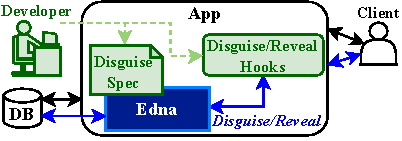
\includegraphics{figs/edna_overview.pdf}
    \caption{Developers write seal specifications and add hooks to invoke Edna
        from the application (green); in normal operation, clients use these
        hooks in the application to seal and reveal their data in the database
        (blue).
    }
  \label{f:edna-overview}
\end{figure}

\begin{figure*}[h]
  \centering
  \begin{subfigure}[h]{0.6\columnwidth}
  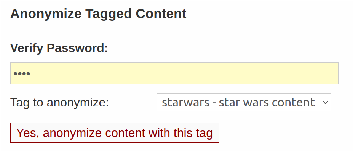
\includegraphics[width=\columnwidth]{figs/lobsters_catanon.pdf}
  \end{subfigure}
  \begin{subfigure}[h]{1.4\columnwidth}
  \begin{lstlisting}[language=Ruby,escapeinside={(*}{*)}]
  def tag_anon
    # instantiate the seal spec with the provided tag to anonymize
    seal_spec = edna.instantiate_spec("tag_anon.json", params[:tag])
    # apply the sealing transformation
    seal_id = edna.apply_seal(@user.id, params[:password], seal_spec)
    # email the seal ID to the user to allow revealing
    SendSealEmail(@user, seal_id)
  end
  \end{lstlisting}
  \end{subfigure}
  \vspace*{-1em}
  \caption{The Lobsters developer adds a hook in the UI and code to perform
      category-based content anonymization.}
  \label{f:lobsters_hook}
  \end{figure*}
\end{comment}

%
Edna supports user data control in web applications using
application-specific \emph{sealing transformations}.
%
To integrate an application with Edna, the developer writes seal
specifications and adds hooks to seal or reveal data using Edna's API.
%(Figure~\ref{f:edna-overview}).
%
Applications (1) register users (human principals) with Edna, (2) invoke Edna to apply
transformations that seal user data, and (3) invoke Edna to reveal that data
when requested.

%%%%%%%%%%%%%%%%%%%%%%%%%%%%%%%%%%%%%%%%%%%%%%%%%%%%%%%%%%%%%%%%%%%%%%%%%%%
(1) Applications register users with a public--private keypair
that either the application or the user's client generates; Edna stores the
public key in its database, while the user remembers the private key for use in
future reveal operations.
%

%
(2) When the application wants to seal some data, it invokes Edna with the
corresponding developer-provided seal specification and any necessary
parameters (such as a user ID).
%
Seal specifications can remove data, modify data (replacing some or all of its
contents with placeholder values), or decorrelate data, replacing
links to users with links to pseudoprincipals (fake users).
%
Edna takes the data it removed or replaced and the connection between
the user and any pseudoprincipals it created, encrypts that data with the user's
public key, and stores the resulting ciphertext---the \emph{sealed
data}---such that it cannot be linked to
the user without the user's private key.
%

%
(3) When a user wishes to reveal their sealed data, they pass credentials
to the application, which calls into Edna to reveal the data.
%
Credentials are application-specific: users may either provide their private
key or other credentials sufficient for Edna to re-derive the private key.
%
Edna gets the sealed data and decrypts it, undoing the changes to the
application database that sealing introduced.

%
Edna provides the developer with sensible default sealing and revealing
semantics (\eg revealing makes sure not to overwrite changes made since
sealing), which the developer can customize via a low-level API provided by
Edna.

%%%%%%%%%%%%%%%%%%%%%%%%%%%%%%%%%%%%%%%%%%%%%%%%%%%%%%%%%%%%%%%%%%%%%%
\head{Threat Model.}
\label{s:threat}
%
Edna assumes well-intentioned developers who write seal specifications
that capture the desired application semantics.
%
Edna seals data according to these specifications, but because some data
must be retained in the database to keep application semantics intact,
Edna cannot protect against inference attacks.
%provide information-theoretic privacy guarantees.
%
Nevertheless, Edna protects a user's \emph{sealed} data against:
%
\begin{enumerate}[nosep]
  \item arbitrary application database accesses (\eg SQL
    injection attacks);
  \item public exposure or other users' ability to view the data through
    the application (\eg compromised accounts, including privileged ones); and
  \item remote code execution with the application's privileges
    (\eg PHP's \texttt{eval()}).
\end{enumerate}
%
Edna guarantees that a user's sealed data is protected unless an attacker
obtains their credentials.
%
While Edna hides the contents of sealed data and relationships between sealed
data and users, it does not hide the existence of sealed data. (An attacker
can see whether a user has sealed some data, but cannot see which sealed data
corresponds to this user.)
%
Some transformations, especially decorrelation, cannot protect against
statistical inference attacks over information still visible in the database.
%
Edna also cannot handle copies of data embedded in other data (\eg quoted
text) or snapshots saved when the data was still in the database.
%
% STANDARD CLAIMS ABOUT CRYPTO ASSUMPTIONS
We make standard assumptions about the security of cryptographic primitives:
attackers cannot break encryption, and keys stored with clients are safe.
%
